\documentclass[pdftex,12pt,letter]{article}
\usepackage{fancyhdr}
\usepackage{enumerate}
\usepackage{tabularx}
\usepackage{graphicx}
\usepackage{array}
\usepackage[justification=justified,singlelinecheck=false]{caption}
\usepackage{placeins}
\pagestyle{fancy}
\makeatletter
  \renewcommand\@seccntformat[1]{\csname the#1\endcsname.\quad}
\makeatother

\newcolumntype {Y}{ >{\raggedright \arraybackslash }X}
\newcommand{\HRule}{\rule{\linewidth}{0.5mm}}
\captionsetup{labelformat=empty}

\begin{document}

\begin{titlepage}
\begin{flushright}
\HRule \\[0.4cm]
{ \bfseries
{\huge Functional Test Requirements\\[1cm]}
{\Large for\\[1cm]}
{\huge CWRUtility\large\\[4cm]}
{\large Prepared by\\Jason Kuster, Stuart Long, and William Ordiway\\[1cm]
Version 1.0\\[1cm]
KOALAA Development\\[1cm]
November 12, 2012}}
\end{flushright}
\end{titlepage}
\tableofcontents{}
\begin{table}[!t]
\caption*{\bfseries Revision History}
\begin{tabularx}{\textwidth }[t]{|l|Y|Y|l|}
\hline
\bfseries Name & \bfseries Date & \bfseries Reasons for Change & \bfseries Version \\ \hline
Long & 9/22/2012 & Initial Draft & 1.0a\\
\hline
\end{tabularx}
\end{table}
\FloatBarrier
\newpage
\clearpage


\lfoot{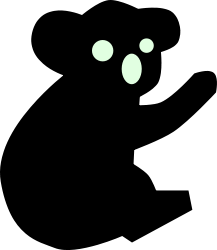
\includegraphics[height=1cm]{DarkKoala.png}}
\end{document}